\documentclass[]{article}

% Imported Packages
%------------------------------------------------------------------------------
\usepackage{amssymb}
\usepackage{amstext}
\usepackage{amsthm}
\usepackage{amsmath}
\usepackage{enumerate}
\usepackage{fancyhdr}
\usepackage[margin=1in]{geometry}
\usepackage{graphicx}
%\usepackage{extarrows}
%\usepackage{setspace}
%\usepackage{xcolor}
\usepackage{color}
\usepackage{float}
\usepackage{url}
%------------------------------------------------------------------------------

% Header and Footer
%------------------------------------------------------------------------------
\pagestyle{plain}  
\renewcommand\headrulewidth{0.4pt}                                      
\renewcommand\footrulewidth{0.4pt}                                    
%------------------------------------------------------------------------------

% Title Details
%------------------------------------------------------------------------------
\title{Deliverable \#1 : Software Requirement Specification (SRS)}
\author{SE 3A04: Software Design II -- Large System Design}
\date{\today}
                            
%------------------------------------------------------------------------------

% Document
%------------------------------------------------------------------------------
\begin{document}

\maketitle	
\noindent{\bf Tutorial Number:} T01\\
{\bf Group Number:} G3 \\
{\bf Group Members:} 
\begin{itemize}
	\item Klisuric, Petar
    \item Bornomala, Anindita
    \item Nielsen, Claire
    \item Nesbitt, Matthew
    \item Lam, Robert 
    \item Rooprai, Mankaran
\end{itemize}

\section*{IMPORTANT NOTES}
\begin{itemize}
	\item Be sure to include all sections of the template in your document regardless whether you have something to write for each or not
	\begin{itemize}
		\item If you do not have anything to write in a section, indicate this by the \emph{N/A}, \emph{void}, \emph{none}, etc.
	\end{itemize}
	\item Uniquely number each of your requirements for easy identification and cross-referencing
	\item Highlight terms that are defined in Section~1.3 (\textbf{Definitions, Acronyms, and Abbreviations}) with \textbf{bold}, \emph{italic} or \underline{underline}
	\item For Deliverable 1, please highlight, in some fashion, all (you may have more than one) creative and innovative features. Your creative and innovative features will generally be described in Section~2.2 (\textbf{Product Functions}), but it will depend on the type of creative or innovative features you are including.
\end{itemize}

\newpage
\section{Introduction}
\label{sec:introduction}
% Begin Section
This SRS will describe the software requiremnets for \textbf{GeoLens}, a community-driven application for identifying
locations based on images, descriptitons and discussions. This document outlines the system's overall purpose, the context for building the application,
functional and non-functional requirements and user iteraction.

\subsection{Purpose}
\label{sub:purpose}
% Begin SubSection
This document serves as a guideline for developers, designers, QA engineers, project managers and other stakeholders, ensuring a clear understanding of the system, including it's objectives, users, expected behavior, and technical constraints.
As the project progresses and changes, the document will provide a baseline from which these changes can be compared. This SRS may also aid in risk identification early in the project lifecycle by outlining dependencies and constraints, allowing managers to prevent risks.
% End SubSection

\subsection{Scope}
\label{sub:scope}
% Begin SubSection
\textbf{GeoLens} is a community and AI driven application designed to identify locations from images. It consists of several individual software products described below.\\

The \textbf{Forum} UI is the primary interface where users interact with \textbf{GeoLens}. It allows users to upload images of locations for identification, view responses, and
engage with the community. If the forum UI can provide ease of use and an interactive experience it will encourage community engagement and bring traffic to the
application. The interface facilitates discussions, displays aggregated predictions, and contains gamification elements such as leaderboards. The forum UI should be accessible
to all users, intuitive to use and respond to user requests within 100 ms. It does not perform image analysis or identification itself but serves as the user’s gateway to the platform.\\

The \textbf{Orchestrator} is responsible for handling submitted images, delegating tasks to experts,
and returning the final result to users. The Orchestrator should coordinate system components concurrently, managing task distribution, monitoring progress, and aggregating responses to ensure quick and accurate results. It handles task prioritization, load balancing, and error recovery while maintaining seamless interactions between users and experts.
The back end does not analyze images directly but functions as the between layer that processes requests and returns items to the forum.\\

The \textbf{Host DBMS} stores user account information, historical user interactions, reputation scores, previously identified locations and leaderboards. It ensures that the system retains valuable data,
in a structured way that is efficiently accessible by other system components. The database should be highly secure, as it contains sensitive user information. The database does not process images or make
identifications but acts as the central location for all platform data. \\

The three \textbf{Experts} are as follows:
\begin{enumerate}
    \item \textbf{GeoKnowr AI}
    \begin{itemize}
        \item Pre-trained image processing model
        \item Predicts coordinates where an image was taken
    \end{itemize}
    \item \textbf{Landmark Recognition}
    \begin{itemize}
        \item Google images API
        \item Search by image to locate a popular landmark
    \end{itemize}
	\item \textbf{Region Specific AI}
	\begin{itemize}
        \item Uses a specialized AI model trained for a specific region
        \item Enhances accuracy for areas with distinct visual features
    \end{itemize}
\end{enumerate}

The primary goal of these experts is to work cohesively to provide an accurate prediction with little delay. \textbf{GeoKnowr} AI aims to deliver an initial estimate
of where an image was taken by assigning coordinates. Then the region specific AI can further refine this prediction by applying localized knowledge. If a landmark is 
present in the image, the Landmark Recognition software should pin point it's location.

\subsection{Definitions, Acronyms, and Abbreviations}
\label{sub:definitions_acronyms_and_abbreviations}
% Begin SubSection
\begin{itemize}
	\item \textbf{GeoLens:} the system being specified
    \item \textbf{GeoKnowr:} pre trained image to coordinates model
	\item \textbf{AI:} Aritficial Intelligence
\end{itemize}
% End SubSection

\label{sub:references}
\begin{thebibliography}{99}
    \bibitem{ref1} Non-functional requirements - the University of Texas at ..., 
    \url{https://personal.utdallas.edu/~chung/SYSM6309/NFR-18-4-on-1.pdf} 
    (accessed Feb. 7, 2025).
    
    \bibitem{ref2} AltexSoft,"Nonfunctional requirements:Examples, types and approaches,"AltexSoft, 
    \url{https://www.altexsoft.com/blog/non-functional-requirements/} 
    (accessed Feb. 7, 2025).
    
    \bibitem{ref3} “Android mobile App Developer tools,” Android Developers, 
    \url{https://developer.android.com/} 
    (accessed Feb. 7, 2025). 
    
    \bibitem{ref4} Office of the Privacy Commissioner of Canada, “Pipeda Fair Information principles,” Office of the Privacy Commissioner of Canada,  \url{https://www.priv.gc.ca/en/privacy-topics/privacy-laws-in-canada /the-personal-information-protection-and-electronic-documents}\\
    \url{-act-pipeda/p_principle/} 
    (accessed Feb. 8, 2025). 
    
     \bibitem{ref5} Google, “Google Play Developer Distribution Agreement,” Google Play,  
    \url{https://play.google/developer-distribution-agreement.html} 
    (accessed Feb. 8, 2025). 
    
    \bibitem{ref6} G. Aspinwall, “A list of 723 bad words to blacklist \& how to use Facebook’s moderation tool,” FrontGate Media,  
    \url{https://www.frontgatemedia.com/a-list-of-723-bad-words-to-blacklist-and-how-}\\
    \url{to-use-facebooks-moderation-tool/}
    (accessed Feb. 8, 2025). 
    
    \bibitem{ref7} Office of the Privacy Commissioner of Canada, “Pipeda Fair Information Principle 1 –- accountability,” Office of the Privacy Commissioner of Canada,
    \url{https://www.priv.gc.ca/en/privacy-topics/privacy-laws-in-canada/the-personal-information-protection-and-electronic-documents}\\
    \url{-act-pipeda/p_principle/principles/p_accountability/} 
    (accessed Feb. 8, 2025). 
   
    \bibitem{ref8} Office of the Privacy Commissioner of Canada, “Pipeda Fair Information Principle 2 –- identifying purposes,” Office of the Privacy Commissioner of Canada,  
    \url{https://www.priv.gc.ca/en/privacy-topics/privacy-laws-in-canada/the-personal-information-protection-and}\\
    \url{-electronic-documents-act-pipeda/p_principle/principles/p_purposes/} 
    (accessed Feb. 8, 2025). 
   
    \bibitem{ref9} Office of the Privacy Commissioner of Canada, “Pipeda Fair Information Principle 3 -– Consent,” Office of the Privacy Commissioner of Canada,  
    \url{https://www.priv.gc.ca/en/privacy-topics/privacy-laws-in-canada/the-personal-information-protection-and-electronic-documents}\\
    \url{-act-pipeda/p_principle/principles/p_consent/} 
    (accessed Feb. 8, 2025). 
    
    \bibitem{ref10} Office of the Privacy Commissioner of Canada, “Pipeda Fair Information Principle 4 -– limiting collection,” Office of the Privacy Commissioner of Canada,  
    \url{https://www.priv.gc.ca/en/privacy-topics/privacy-laws-in-canada/the-personal-information-protection-and-electronic-documents-}\\
    \url{act-pipeda/p_principle/principles/p_collection/} 
    (accessed Feb. 8, 2025). 
    
    \bibitem{ref11} Office of the Privacy Commissioner of Canada, “Pipeda Fair Information Principle 5 –- limiting use, disclosure, and retention,” Office of the Privacy Commissioner of Canada,  \url{https://www.priv.gc.ca/en/privacy-topics/privacy-laws-in-canada/the-personal}\\
    \url{-information-protection-and-electronic-documents-act-pipeda/p_principle/principles/p_use/} 
    (accessed Feb. 8, 2025). 
    
    \bibitem{ref12} Office of the Privacy Commissioner of Canada, “Pipeda Fair Information Principle 7 –- Safeguards,” Office of the Privacy Commissioner of Canada,  
    \url{https://www.priv.gc.ca/en/privacy-topics/privacy-laws-in-canada/the-personal-information-protection-and-electronic-documents}\\
    \url{-act-pipeda/p_principle/principles/p_safeguards/} 
    (accessed Feb. 8, 2025). 
    
    \bibitem{ref13} International Organization for Standardization, “ISO/IEC 42001:2023,” ISO,  
    \url{https://www.iso.org/standard/81230.html} 
    (accessed Feb. 8, 2025). 
    
    \bibitem{ref14} Android Studio, “Core app quality  :  App quality  :  android developers,” Android Developers,  
    \url{https://developer.android.com/docs/quality-guidelines/core-app-quality} 
    (accessed Feb. 8, 2025). 
\end{thebibliography}
% End SubSection

\subsection{Overview}
\label{sub:overview}
% Begin SubSection
Section 2 aims to put the value of \textbf{GeoLens} into perspective, relating and contrasting it to other similar products that currently exist.
It should also provide a summary of the primary functions of the application and a description of the expected users. This should provide readers with a general understanding
of the system, and how users are expected to intereact with it. Finally, constraints and assumptions are listed to clarify the scope of the application and the context in which it operated.\\\\
Section 3 presents a use case digram outlining the main functionality and interactions with stakeholders.\\\\
Section 4 is a detailed overview of the functional requirements, discussing what the system will do. These requirements will be organized in terms of 
business events, viewpoints and scenarios. This provides a structured understanding of the system in various contexts. \\\\
Finally, section 5 describes the Non-Functional Requirements, focusing on how the system aims to be a valuable service. This section provides a rationale for each requirement, explaining their necessity and benefits.

% End Section

\section{Overall Product Description}
\label{sec:overall_description}
% Begin Section

% \begin{itemize}
% 	\item This section should describe the general factors that affect the product and its requirements. 
% 	\item It does not state specific requirements.
% 	\item It provides a \emph{background} for those requirements and makes them easier to understand.
% \end{itemize}


\subsection{Product Perspective}
\label{sub:product_perspective}

\noindent \textbf{GeoLens} is a mobile game guessing app developed for the Android platform. A similar product is GeoGuessr, which allows users to guess the location of randomly given locations from a Google Street View. However, GeoLens requires a user to submit a picture of a location they wish to identify. The application will consult three specialized experts: a lightweight AI called \textbf{GeoKnowr} which is based off of GeoGuessr, a Landmark Recognition service, and a region-specific generative AI. Each expert will return a confidence level and if the confidence level meets a predefined threshold of 70\%, then that expert's response will be returned in the same order as above.\\

\noindent In addition to the AI-driven location identification, \textbf{GeoLens} has a unique gameplay feature with competition modes, where players can play against each other individually, with real-time score tracking and leaderboards. Additionally, the product will allow users to create and modify profiles that will be used in the app. This means that a log-in and sign-up feature will be required.\\

\noindent The system architecture consists of multiple layers. Firstly, there is the Host DBMS layer for storing user profiles, previously submitted images, as well as game history. Secondly, there is the Orchestrator Wrapper which is responsible for managing images, managing accounts, and allowing users to engage in competition mode. Next is the external AI layer which is where the Image Identification Service module calls on to identify photos, where it calls upon a confidence evaluator, which aggregates responses from multiple AI models to determine the most accurate result. Lastly, the Figure UI layer is where the user interacts with \textbf{GeoLens}.\\

\begin{figure}[h]
    \centering
    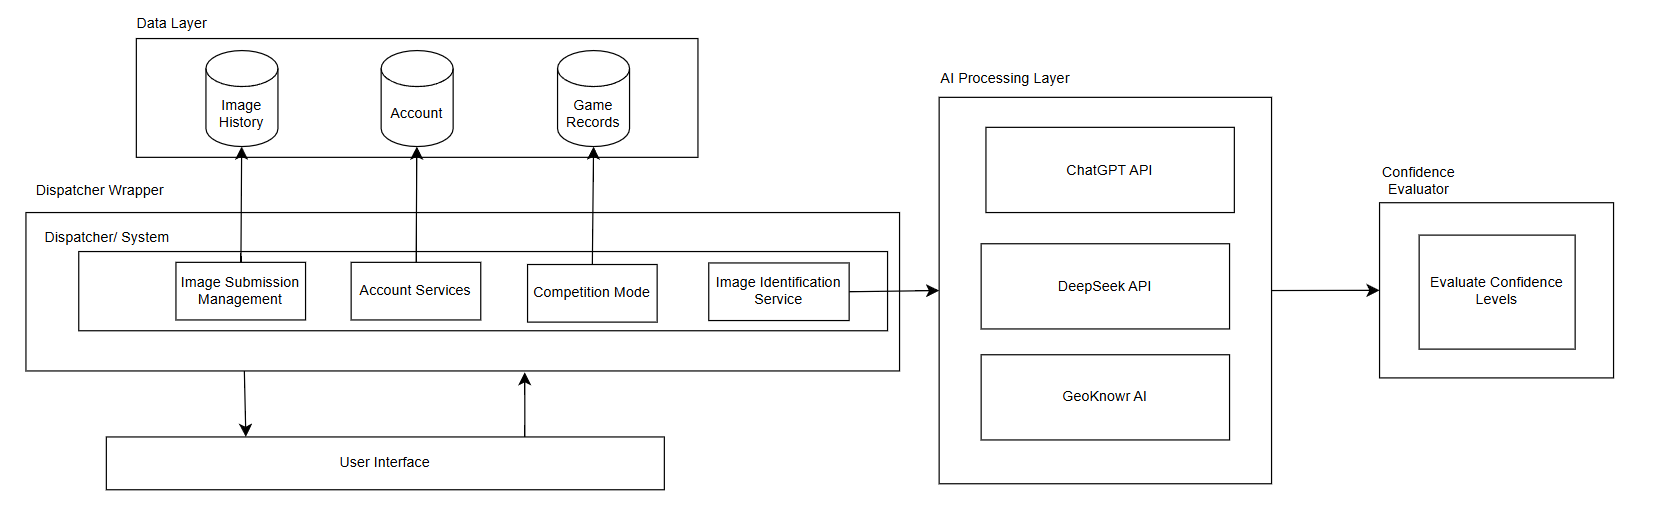
\includegraphics[width=1\linewidth]{system_diagram.png}
    \caption{System Architecture Diagram}
    \label{fig:system_diagram}
\end{figure}

\subsection{Product Functions}
\label{sub:product_functions}
% Begin SubSection

\noindent There will be 4 modules in the product: Image Management, Account Services, Competition Mode, and the Image Identification Service. The major functions of the software in Image  Management include uploading images, allowing users in Competition Mode to see the picture of a location and make a guess, providing additional context for images, and sending images for AI processing. Within Account Services, there are functions of creating and updating accounts, and logging in. \textbf{Competition Mode} is the innovative feature in this application, which allows users to engage in challenges, view leaderboards, and compete in multiplayer mode. Lastly, Image Identification Services involves AI models processing images, evaluating their confidence, and returning predictions for the location.\\

\noindent The following table outlines the major functions within each module:

\noindent
\begin{tabular}{| p{3cm} | p{13cm} |} % Adjust column widths
    \hline
    \raggedright \textbf{Modules} & \textbf{Functions} \\
    \hline
    \raggedright \textbf{Image Management} & 
    • Upload Image \newline 
    \makebox[5mm]{} - Allows users to submit an image for location identification. \vspace{5pt}\newline
    • Provide Additional Context \newline 
    \makebox[5mm]{} - Users can enter optional metadata (e.g., approximate location, description). \vspace{5pt}\newline
    • Return Image Guess Result to User in Competition Mode \newline 
    \makebox[5mm]{} - Users in Competition Mode see the picture of a location and make a guess. \vspace{5pt}\newline
    • Send to AI Processing \newline 
    \makebox[5mm]{} - Forwards submitted images to AI experts for analysis. \\
    \hline
    \raggedright \textbf{Account Services} & 
    • Create Account \newline 
    \makebox[5mm]{} - Allows users to register a new account. \vspace{5pt}\newline
    • Login/Logout \newline 
    \makebox[5mm]{} - Users can authenticate themselves to access features. \vspace{5pt}\newline
    • Manage Profile \newline 
    \makebox[5mm]{} - Users can update their profile information. \\
    \hline
    \raggedright \textbf{Competition Mode} & 
    • Start Challenge \newline 
    \makebox[5mm]{} - Allows users to enter a competitive mode where they try to guess locations. \vspace{5pt}\newline
    • Leaderboard \newline 
    \makebox[5mm]{} - Tracks and ranks users based on their accuracy.\vspace{5pt} \newline
    • Multiplayer Mode \newline 
    \makebox[5mm]{} - Allows users to compete against others in real-time. \\
    \hline
    \raggedright \textbf{Image Identification Services} & 
    • AI Processing \newline 
    \makebox[5mm]{} - Uses multiple AI models (\textbf{GeoKnowr} AI, Landmark Recognition, Region-Specific AI) to analyze images. \vspace{5pt}\newline
    • Confidence Evaluation \newline 
    \makebox[5mm]{} - Aggregates responses from AI models and determines the most accurate result. \vspace{-4pt}\newline
    • Return Prediction \newline 
    \makebox[5mm]{} - Displays the predicted location to the user. \\
    \hline
\end{tabular}

% \noindent
\begin{figure}[H]
    \centering
    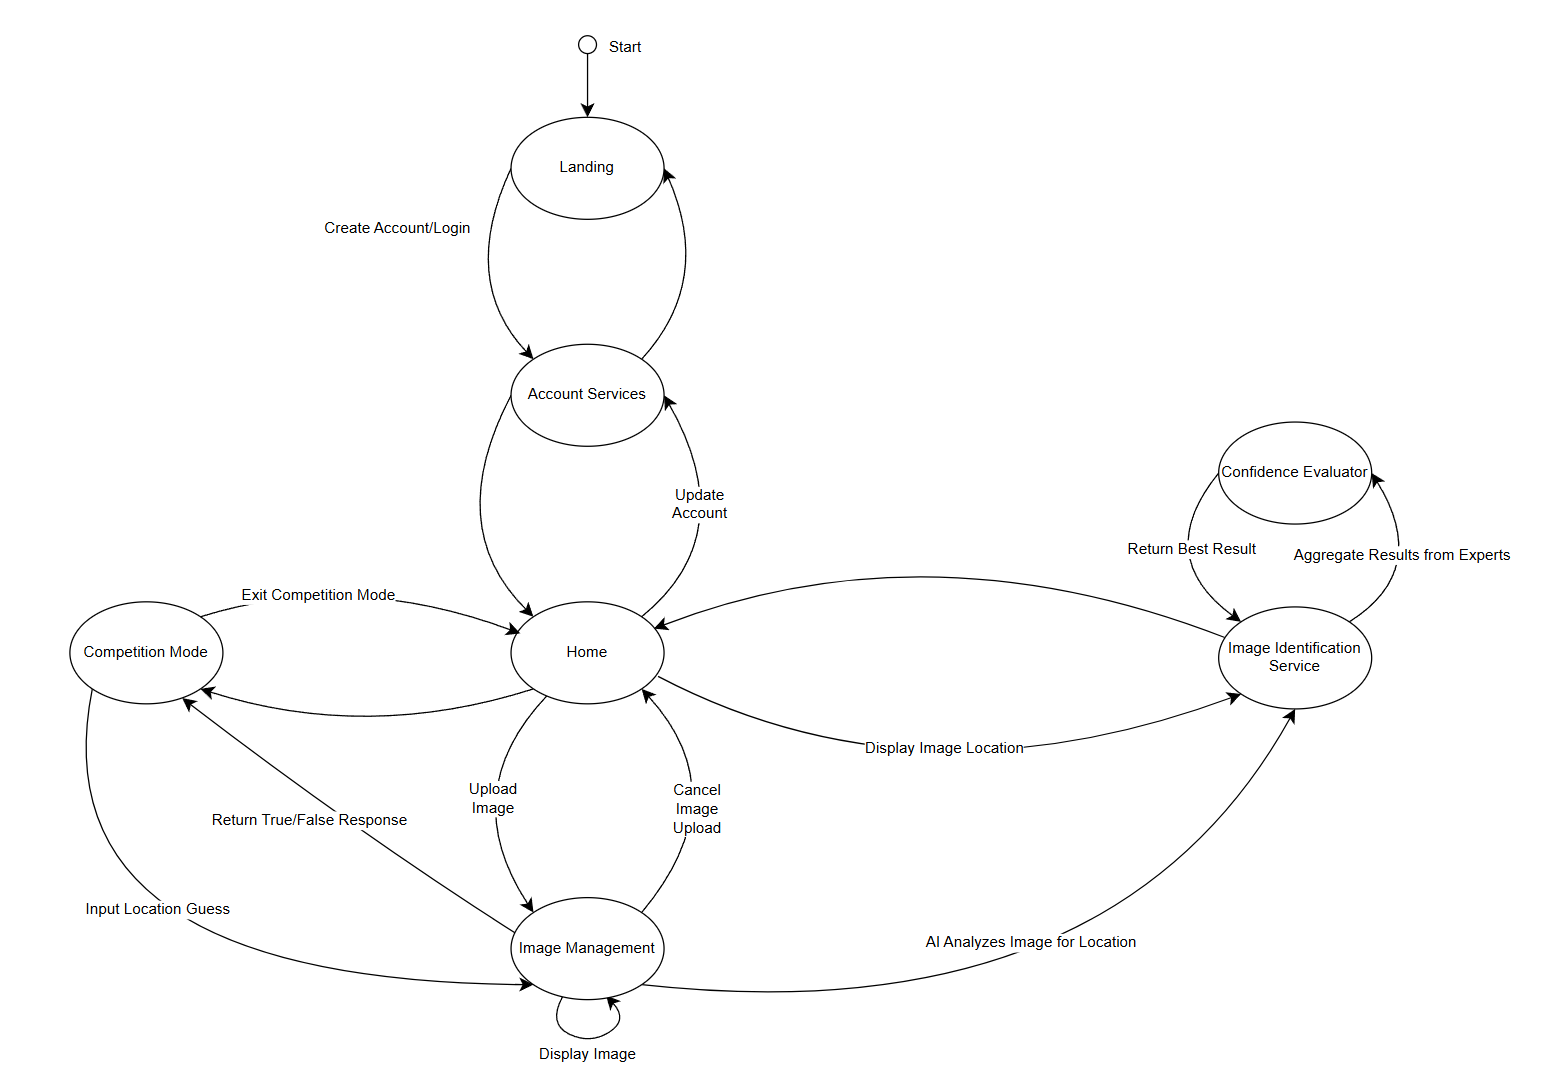
\includegraphics[width=1.1\linewidth]{state_diagram.png}
    \caption{State Diagram}
    \label{fig:state_diagram}
\end{figure}

% End SubSection

\subsection{User Characteristics}
\label{sub:user_characteristics}
% Begin SubSection
The app is meant to be a user-friendly app and as a result has the following expected qualifications of its users:\\ \\
1. Education Level: Basic Literacy and Geographical knowledge
\begin{itemize}
	\item A person with basic literacy skills of reading and writing should be able to utilize
		this app without any difficulties.
	\item A person with basic geographical knowledge of the divison of the world into continents, countries, and regions
		should be able to utilize this app without any difficulties.
\end{itemize}
2. Experience: Any
\begin{itemize}
	\item Since the app is meant to be user-friendly, someone who is using the app for the very first time
		should be able to do so without any major problems.
\end{itemize}
3. Technical Expertise: Basic knowledge of smartphone usage
\begin{itemize}
	\item A person having basic experience with the usage of a smartphone should be able to easily use the app.
\end{itemize}

% End SubSection

\subsection{Constraints}
\label{sub:constraints} \medskip
% Begin SubSection
1. \textbf{Budget: }The budget allocated to the project will have a great affect on which technologies may be used
in the development of the app, as well as limiting the external integrations that can be used. The indicated
budget for the project is \$0.\medskip \\
2. \textbf{Time: }The time allotted for the project with have a significant affect on the feasible scope of the
project. Consequently, this limits the number and quality of features that can be integrated into the app.
% End SubSection

\subsection{Assumptions and Dependencies}
\label{sub:assumptions_and_dependencies}
% Begin SubSection
1. Assume that pictures of locations will be able to be located to at minimum country level accuracy.\\
2. Assume that users encounter pictures of unknown origin (no information about where it was taken).\\
3. Assume that users wish to know where pictures of unknown origin were taken.\\
4. Assume that the processing of unauthorized photos of public spaces are legal in all regions in which the app operates. \medskip \\
Other assumptions that, if it fails to hold, could require a change to the requirements:\\
1. A recent (released within 3 years) version of the Andriod operating system will be available on the device.\\
2. The device will have internet access if the user wishes to use the app.\\
3. The app will have access to an on-device photo library if the user wishes to upload a photo.\\
4. Assume all API dependencies are fully functional during the operation of the product.
%\begin{itemize}
%	\item List any assumptions you made in interpreting what the software being developed is aiming to achieve
%	\item List any other assumptions you made that, if it fails to hold, could require you to change the requirements
	%\item List each of the factors that affect the requirements stated in the SRS
	%\item These factors are not design constraints on the software but are, rather, any changes to them that can affect the requirements in the SRS
%	\begin{itemize}
%		\item \textbf{Example}: An assumption may be that a specific operating system will be available on the hardware designated for the software product. If, in fact, the operating system is not available, the SRS would then have to change accordingly.
%	\end{itemize}
%\end{itemize}
% End SubSection

\subsection{Apportioning of Requirements}
\label{sub:apportioning_of_requirements}
% Begin SubSection
1. Further language capabilities
\begin{itemize}
	\item The software will be developed only in English for the first version
		of the system.
\end{itemize}
2. User rating/rank based on guess accuracy
\begin{itemize}
	\item Users will be able to guess on other user's posts as to where
		they think it is (This does \textbf{not} affect the expert determination
		and is simply to add game-like mechanics). In a future version of the software,
		each user will have a rating/rank
		based on how close their guesses are to the expert determination.
\end{itemize}
3. No question limit for paid tier
\begin{itemize}
	\item In a future version of the software, users would be able to
		purchase a paid premium tier to be able to ask as many questions
		per day as they'd like.
\end{itemize}
%\begin{itemize}
%	\item Identify requirements that may be delayed until future versions of the system
%\end{itemize}
% End SubSection

% End Section
\section{Use Case Diagram}
\label{sec:use_case_diagram}
% Begin Section
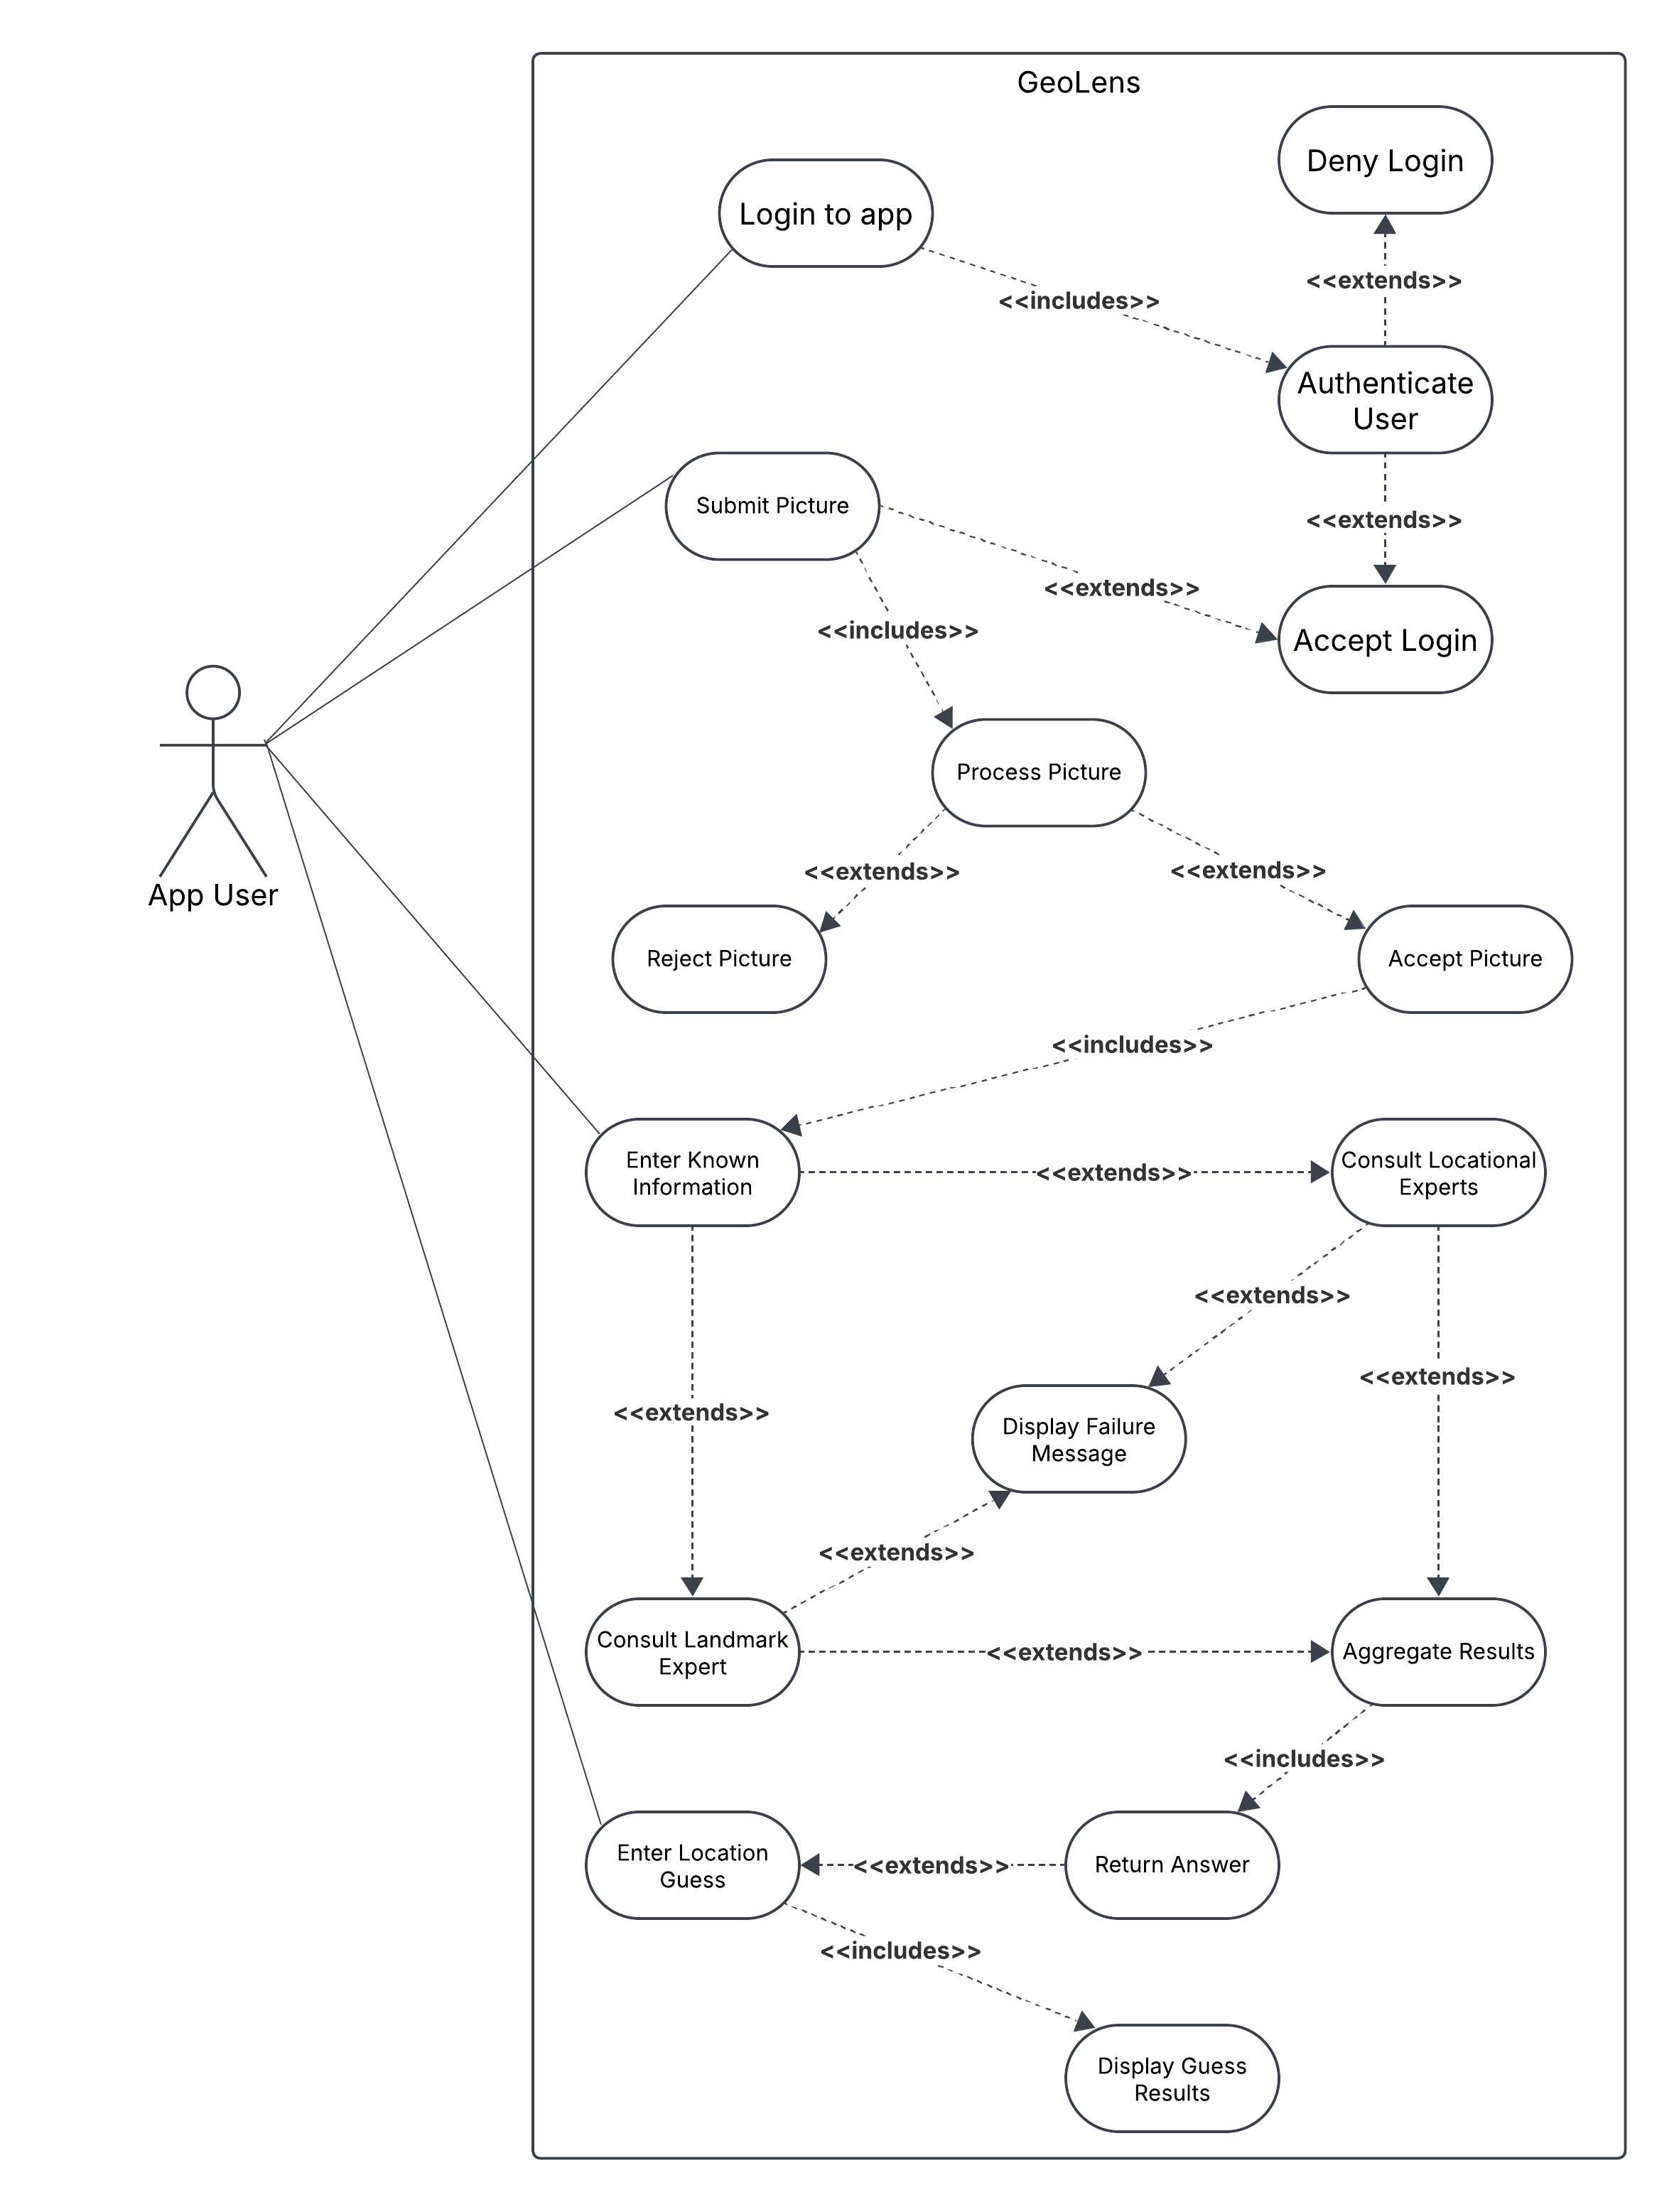
\includegraphics[scale=0.8]{usecase}
%\begin{itemize}
%	\item Provide the use case diagram for the system being developed.
%	\item You do not need to provide the textual description of any of the use cases here (these will be specified under "Highlights of Functional Requirements").
%	\item Provide \emph{one} use case diagram for the most important Business Event.
%	\item The text of all use cases will be specified under "Highlights of Functional Requirements"
%\end{itemize}
%In this section, select the most important Business Event that your system responds to and give its use case diagram.  Only one use case diagram is needed.  Give a brief textual description of the use case without repeating what is in the scenarios of the corresponding Business Event.

%
%
%
%This section should provide a use case diagram for your application. 
%\begin{enumerate}[a)]
%	\item Each use case appearing in the diagram should be accompanied by a text description. 
%\end{enumerate}
%% End Section

\section{Highlights of Functional Requirements}
\label{sec:functional_requirements}
% Begin Section
\begin{itemize}
	\item Specify all use cases (or other scenarios triggered by other events), organized by Business Event. 
	\item For each Business Event, show the scenario from every Viewpoint. You should have the same set of Viewpoints across all Business Events. If a Viewpoint doesn't participate, write N/A so we know you considered it still. You can choose how to present this - keep in mind it should be easy to follow. 
	\item At the end, combine them all into a Global Scenario.
	%\item Specify the "use cases" (or other triggering events) organized by Business Event. (The Global Scenario is what you might think of as a use case). Be sure to consider Business Events that aren't just triggered by users with goals (e.g. something happens in the environment that your system needs to respond to)
	\item Your focus should be on what the system needs to do, not how to do it. Specify it in enough detail that it clearly specifies what needs to be accomplished, but not so detailed that you start programming or making design decisions.
	\item Keep the length of each use case (Global Scenario) manageable. If it's getting too long, split into sub-cases.
	\item You are \emph{not} specifying a complete and consistent set of functional requirements here. (i.e. you are providing them in the form of use cases/global scenarios, not a refined list). For the purpose of this project, you do not need to reduce them to a list; the global scenarios format is all you need.
	\item Red text below is just to highlight where you need to insert a scenario - don't actually write it all in red.
\end{itemize}

\noindent {\bf Main Business Events:} List out all the main business events you are presenting. If you sub-divided into smaller ones, you don't need to include the smaller ones in this list.\\

\noindent {\bf Viewpoints:} List out all the viewpoints you will be considering.\\

\noindent {\bf Interpretation:} Specify any liberties you took in interpreting business events, if necessary.\\

\begin{enumerate}[{\bf BE1.}]
	\item User Submits a Picture (not region specific)
        \\ Pre-Condition: The user must have an account and a working app with internet connection. 
		\begin{enumerate}[{\bf VP1.}]
			\item User \\
				Main Success Scenario
                    \begin{enumerate}[{1.}]
                        \item User opens the app on their mobile device.
                        \item The app prompts the user to enter their login information.
                        \item User enters their login information.
                        \item System authenticates the user. 
                        \item System gives user options to choose from (Submit a Picture, Submit a Landmark). 
                        \item User chooses “Submit a Picture”. 
                        \item Systems prompts the user to upload a picture within the resolution and format requirements.
                        \item User uploads picture.
                        \item System prompts the user to include a general region where the picture is from. 
                        \item User does not input a region. 
                        \item System prompts the user to include comments on where the image is from (Instagram, family photo, etc). 
                        \item User adds comments.
                        \item User submits the post.
                        \item System sends data to the general AI.
                        \item The general AI returns an approximate location, which is passed to the region specific AI.
                        \item The region-specific AI returns an answer. 
                        \item Answer is displayed to the user. \\
                    \end{enumerate}
                    Secondary Scenario \\
                    4.i. System fails to authenticate user. Login failed, retry form step 3. \\
                    8.i. User uploads a photo outside quality/format requirements. Retry from step 8.\\ 
                    14.i. System fails to send post to AI. \\
                    14.ii. The post is not sent, but the data is saved. Retry from step 13. \\
                    14.ii. The post is not sent and information is not saved. Retry from step 7. \\
                    15.i. General AI cannot return an answer. Error page is displayed. 
                    16.i. The region-specific AI cannot return an answer. The general answer returned by the general AI is returned to the user.
                    
			\item Customer Support \\
				4.i. On failure, system prompts user with contact          information for Customer Support. \\
                    8.i. On failure, system displays image parameters and prompts user with contact information for Customer Support. \\
                    14.i. System displays an error page with contact information for Customer Support. \\
	            14.ii. System prompts user to retry send, or contact       Customer Support. \\
	            14.ii. System prompts user to re-input image and data,     or contact Customer Support. \\
		\end{enumerate}
		{\bf Global Scenario:}\\
            Pre-Condition: The user must have an account and a working app with internet connection. 
		      \begin{enumerate}[{1.}]
                    \item User opens the app on their mobile device. 
                    \item The app prompts the user to enter their login information.
                    \item User enters their login information.
                    \item System authenticates the user. 
                    \item System gives user options to choose from (Submit a Picture, Submit a Landmark).  
                    \item User chooses “Submit a Picture”. 
                    \item Systems prompts the user to upload a picture within the resolution and format requirements.
                    \item User uploads picture.
                    \item System prompts the user to include a general region where the picture is from. 
                    \item User does not input a region. 
                    \item System prompts the user to include comments on where the image is from (Instagram, family photo, etc). 
                    \item User adds comments.
                    \item User submits the post.
                    \item System sends data to the general AI.
                    \item The general AI returns an approximate location, which is passed to the region specific AI.
                    \item The region-specific AI returns an answer. 
                    \item Answer is displayed to the user. \\
                \end{enumerate}
                    Secondary Scenario \\
                    4.i. System fails to authenticate the user. 
                    System prompts user with contact information for Customer Support. User can retry from step 3. \\
                    8.i. User uploads a photo outside quality/format requirements. System displays image parameters. System prompts user with contact information for Customer Support.User can retry from step 8. \\
                    14.i. System fails to send post to the forum. \\
	            14.ii. 	The post is not sent, but the data is saved. \\
                    System prompts user to contact Customer Support. User can retry from step 13. \\
	            14.ii. 	The post is not sent and information is not        saved.\\ 
                    System prompts user to contact Customer Support. User can retry from step 7. \\
                    15.i. General AI cannot return an answer. Error page is displayed. \\ 
                    16.i. The region-specific AI cannot return an answer. The general answer returned by the general AI is returned to the user.\\
	\item User Submits a Picture (region specific)
	\begin{enumerate}[{\bf VP1.}]
		\item User \\
		Main Success Scenario
                    \begin{enumerate}[{1.}]
                        \item User opens the app on their mobile device.
                        \item The app prompts the user to enter their login information.
                        \item User enters their login information.
                        \item System authenticates the user. 
                        \item System gives user options to choose from (Submit a Picture, Submit a Landmark). 
                        \item User chooses “Submit a Picture”. 
                        \item Systems prompts the user to upload a picture within the resolution and format requirements.
                        \item User uploads picture.
                        \item System prompts the user to include a general region where the picture is from. 
                        \item User inputs a region. 
                        \item System prompts the user to include comments on where the image is from (Instagram, family photo, etc). 
                        \item User adds comments.
                        \item User submits the post.
                        \item System sends data to the appropriate region-specific AI. 
                        \item The region-specific AI returns an answer. 
                        \item Answer is displayed to the user. \\
                    \end{enumerate}
                    Secondary Scenario \\
                    4.i. System fails to authenticate user. Login failed, retry form step 3. \\
                    8.i. User uploads a photo outside quality/format requirements. Retry from step 8.\\ 
                    14.i. System fails to send post to AI. \\
                    14.ii. The post is not sent, but the data is saved. Retry from step 13. \\
                    14.ii. The post is not sent and information is not saved. Retry from step 7. \\
                    15.i. The region-specific AI cannot return an answer. Error page is displayed. \\
			\item Customer Support \\
				4.i. On failure, system prompts user with contact          information for Customer Support. \\
                    8.i. On failure, system displays image parameters and prompts user with contact information for Customer Support. \\
                    14.i. System displays an error page with contact information for Customer Support. \\
	            14.ii. System prompts user to retry send, or contact       Customer Support. \\
	            14.ii. System prompts user to re-input image and data,     or contact Customer Support. \\
		\end{enumerate}
		{\bf Global Scenario:}\\
            Pre-Condition: The user must have an account and a working app with internet connection. 
		      \begin{enumerate}[{1.}]
                    \item User opens the app on their mobile device. 
                    \item The app prompts the user to enter their login information.
                    \item User enters their login information.
                    \item System authenticates the user. 
                    \item System gives user options to choose from (Submit a Picture, Submit a Landmark).  
                    \item User chooses “Submit a Picture”. 
                    \item Systems prompts the user to upload a picture within the resolution and format requirements.
                    \item User uploads picture.
                    \item System prompts the user to include a general region where the picture is from. 
                    \item User inputs a region. 
                    \item System prompts the user to include comments on where the image is from (Instagram, family photo, etc). 
                    \item User adds comments.
                    \item User submits the post.
                    \item System sends data to the appropriate region-specific AI. 
                    \item The region-specific AI returns an answer. 
                    \item Answer is displayed to the user. \\
                \end{enumerate}
                    Secondary Scenario \\
                    4.i. System fails to authenticate the user. 
                    System prompts user with contact information for Customer Support. User can retry from step 3. \\
                    8.i. User uploads a photo outside quality/format requirements. System displays image parameters. System prompts user with contact information for Customer Support.User can retry from step 8. \\
                    14.i. System fails to send post to the forum. \\
	            14.ii. 	The post is not sent, but the data is saved. \\
                    System prompts user to contact Customer Support. User can retry from step 13. \\
	            14.ii. 	The post is not sent and information is not        saved.\\ 
                    System prompts user to contact Customer Support. User can retry from step 7. \\
                    15.i The region-specific AI cannot return an answer. Error page is displayed. \\

		\item User Submits a Landmark
		\begin{enumerate}[{\bf VP1.}]
		\item User \\
		Main Success Scenario
                    \begin{enumerate}[{1.}]
                        \item User opens the app on their mobile device.
                        \item The app prompts the user to enter their login information.
                        \item User enters their login information.
                        \item System authenticates the user. 
                        \item System gives user options to choose from (Submit a Picture, Submit a Landmark). 
                        \item User chooses “Submit a Landmark”. 
                        \item Systems prompts the user to upload a picture within the resolution and format requirements.
                        \item User uploads picture.
                        \item System prompts the user to include comments on where the image is from (Instagram, family photo, etc). 
                        \item User adds comments.
                        \item User submits the post.
                        \item System sends data to the landmark-focused AI. 
                        \item The landmark-focused AI returns an answer. 
                        \item Answer is displayed to the user. \\
                    \end{enumerate}
                    Secondary Scenario \\
                    4.i. System fails to authenticate user. Login failed, retry form step 3. \\
                    8.i. User uploads a photo outside quality/format requirements. Retry from step 8.\\ 
                    12.i. System fails to send post to AI. \\
                    12.ii. The post is not sent, but the data is saved. Retry from step 11. \\
                    12.ii. The post is not sent and information is not saved. Retry from step 7. \\
                    13.i. The landmark-focused AI cannot return an answer. Error page is displayed. \\
			\item Customer Support \\
				4.i. On failure, system prompts user with contact          information for Customer Support. \\
                    8.i. On failure, system displays image parameters and prompts user with contact information for Customer Support. \\
                    12.i. System displays an error page with contact information for Customer Support. \\
	            12.ii. System prompts user to retry send, or contact       Customer Support. \\
	            12.ii. System prompts user to re-input image and data,     or contact Customer Support. \\ 
		\end{enumerate}
		{\bf Global Scenario:}\\
            Pre-Condition: The user must have an account and a working app with internet connection. 
		      \begin{enumerate}[{1.}]
                    \item User opens the app on their mobile device. 
                    \item The app prompts the user to enter their login information.
                    \item User enters their login information.
                    \item System authenticates the user. 
                    \item System gives user options to choose from (Submit a Picture, Submit a Landmark).  
                    \item User chooses “Submit a Landmark”. 
                    \item Systems prompts the user to upload a picture within the resolution and format requirements.
                    \item User uploads picture.
                    \item System prompts the user to include comments on where the image is from (Instagram, family photo, etc). 
                    \item User adds comments.
                    \item User submits the post.
                    \item System sends data to the landmark-focused AI. 
                \end{enumerate}
                    Secondary Scenario \\
                    4.i. System fails to authenticate the user. 
                    System prompts user with contact information for Customer Support. User can retry from step 3. \\
                    8.i. User uploads a photo outside quality/format requirements. System displays image parameters. System prompts user with contact information for Customer Support.User can retry from step 8. \\
                    12.i. System fails to send post to the forum. \\
	            12.ii. 	The post is not sent, but the data is saved. \\
                    System prompts user to contact Customer Support. User can retry from step 11. \\
	            12.ii. 	The post is not sent and information is not        saved.\\ 
                    System prompts user to contact Customer Support. User can retry from step 7. \\
                    13.i. The landmark-focused AI cannot return an answer. Error page is displayed. \\

	\end{enumerate}
%End Section

\section{Non-Functional Requirements}
\label{sec:non-functional_requirements}


\begin{itemize}
	\item For each non-functional requirement, provide a justification/rationale for it.\\
	{\bf Example:} \\
	SC1. \emph{The device should not explode in a customer’s pocket.}\\
	{\bf Rationale:} Other companies have had issues with the batteries they used in their phones randomly exploding [insert citation]. This causes a safety issue, as the phone is often carried in a person's hand or pocket.	
	\item If you need to make a guess because you couldn't really talk to stakeholders, you can say "We imagined stakeholders would want...because..."
	\item Each requirement should have a unique label/number for it.
	\item In the list below, if a particular section doesn't apply, just write N/A so we know you considered it.
\end{itemize}

% Begin Section
\subsection{Look and Feel Requirements}
\label{sub:look_and_feel_requirements}
% Begin SubSection

\subsubsection{Appearance Requirements}
\label{ssub:appearance_requirements}
% Begin SubSubSection
\begin{enumerate}[{LF-A}1. ]
	\item The system shall have a minimalistic and clean UI.
	
	{\bf Rationale:} A minimalistic and clean UI reduces visual clutter and will allow users to quickly interact with the app while avoiding unnecessary distractions.
	\item All images in the system must be high-quality with the resolution well-adjusted.
	
	{\bf Rationale:} High-quality images ensure a visually appealing and professional user experience. Low-resolution or poorly adjusted images may lead to confusion of the exact location users are looking for, and may reduce the app's credibility and engagement.
	\item The system shall use a consistent and legible font.
	
	{\bf Rationale:} Using a clear and legible font improves readability for users and ensures they can properly navigate the app while reducing extra cognitive strain when reading.
\end{enumerate}
% End SubSubSection

\subsubsection{Style Requirements}
\label{ssub:style_requirements}
% Begin SubSubSection
\begin{enumerate}[{LF-S}1. ]
	\item The system shall have both a light and dark mode option.
	
	{\bf Rationale:} Multiple theme modes provide flexibility and comfort for users, depending on which mode they prefer. Many users prefer dark mode for visual comfort, while others use light mode as either the default theme or in bright environments.
	\item The system must follow a gamified design and have visually appealing elements (ex. Leaderboard, user profile).
	
	{\bf Rationale:} The app has an additional game feature. Users are given an image of a location and are tasked with guessing the location. The gamified design is consistent with this feature and enhances user engagement by making the experience interactive and fun.
	\item The system must scale to the size of the screen.
		
	{\bf Rationale:} Users may have various types and sizes of devices when accessing the app, as such it is important the system scales to fit the screen size to optimize the layout and consistency of the app.
	\item The system must use consistent spacing and padding between elements.
	
	{\bf Rationale:} Proper spacing between elements improves readability and makes it harder for users to be distracted by visual inconsistencies.
\end{enumerate}
% End SubSubSection

% End SubSection

\subsection{Usability and Humanity Requirements}
\label{sub:usability_and_humanity_requirements}
% Begin SubSection

\subsubsection{Ease of Use Requirements}
\label{ssub:ease_of_use_requirements}
% Begin SubSubSection
\begin{enumerate}[{UH-EOU}1. ]
	\item The system's buttons shall be big and bright in colour.
		
	{\bf Rationale:} The app's buttons would be easy to tap, and larger and brighter buttons would ensure that users can comfortably interact with them, especially on smaller screens.
	\item The system shall allow users to complete the identification of a location within four steps.
		
	{\bf Rationale:} By reducing the number of steps required to complete the system's primary task (the main motivation for downloading the app), users will experience less frustration and an efficient and simple app design.
	\item The system shall allow users to report incorrect results through a feedback tool in the application.
	
	{\bf Rationale:} Allowing users a method to report incorrect results encourages them to increase engagement with the app. This also helps maintain accuracy when providing location solutions to users, enhancing the app's reliability and user trust.
\end{enumerate}
% End SubSubSection

\subsubsection{Personalization and Internationalization Requirements}
\label{ssub:personalization_and_internationalization_requirements}
% Begin SubSubSection
\begin{enumerate}[{UH-PI}1. ]
	\item The system must be able to support multiple languages.
		
	{\bf Rationale:} This feature enhances user experience by providing localized content, allowing users to interact with the app in their preferred language.
	\item The system shall allow the user to select between the metric or imperial system to display information.
	
	{\bf Rationale:} Different regions use different measurement systems, improving usability on a wider scale.
\end{enumerate}
% End SubSubSection

\subsubsection{Learning Requirements}
\label{ssub:learning_requirements}
% Begin SubSubSection
\begin{enumerate}[{UH-L}1. ]
	\item The system shall have a basic tutorial for navigating through the features, which automatically executes the first time a user opens the app and is available at all times within the app.
		
	{\bf Rationale:} A built-in tutorial ensures that new users can quickly understand how to navigate the app’s features without overwhelming them. Having the option to review the tutorial enhances usability and accessibility for users who may have forgotten certain functions.
	\item The system shall provide short descriptions when the user presses and holds key features, that automatically fade after a short period.
	
	{\bf Rationale:} Users should be able to learn how basic functionalities work without exiting the app and using external guides.
\end{enumerate}
% End SubSubSection

\subsubsection{Understandability and Politeness Requirements}
\label{ssub:understandability_and_politeness_requirements}
% Begin SubSubSection
\begin{enumerate}[{UH-UP}1. ]
	\item The system shall hide information and aspects of the app construction that are necessary for the user to interact with [1].
		
	{\bf Rationale:} Hiding unnecessary technical details and background processes simplifies the user experience, making the app more intuitive and user-friendly [1].
	\item The system shall provide positive engagement with the user when they successfully identify a location.
	
	{\bf Rationale:} Positive reinforcement encourages users to continue to engage with the app and makes the experience more enjoyable and rewarding.
\end{enumerate}
% End SubSubSection

\subsubsection{Accessibility Requirements}
\label{ssub:accessibility_requirements}
% Begin SubSubSection
\begin{enumerate}[{UH-A}1. ]
	\item The system must be compatible with screen readers.
		
	{\bf Rationale:} Compatibility with screen readers supports visually impaired users and improves inclusivity and accessibility for a wider range of users.
	\item The system shall allow built-in zoom-in and zoom-out features.
		
	{\bf Rationale:} Zoom features improve accessibility by allowing users to adjust content visibility according to their needs.
	\item The system shall provide high-contrast options that are colorblind-friendly.
	
	{\bf Rationale:} High-contrast options ensure that users with colour vision deficiencies can comfortably use the app.
\end{enumerate}
% End SubSubSection

% End SubSection

\subsection{Performance Requirements}
\label{sub:performance_requirements}
% Begin SubSection

\subsubsection{Speed and Latency Requirements}
\label{ssub:speed_and_latency_requirements}
% Begin SubSubSection
\begin{enumerate}[{PR-SL}1. ]
	\item The system shall have a basic app response time of no longer than 3 seconds [2].
		
	{\bf Rationale:} According to Google recommendations for performance requirements, apps with a response time longer than 3 seconds lose over half of user engagement [2]. As such, the app must process and return information fast.
	\item The system shall return location identification results within 5 seconds.
	
	{\bf Rationale:} The system must complete its basic functions quickly, as users expect fast responses. Delays of more than a few seconds may lead to frustration and lower user engagement.
\end{enumerate}
% End SubSubSection

\subsubsection{Safety-Critical Requirements}
\label{ssub:safety_critical_requirements}
% Begin SubSubSection
\begin{enumerate}[{PR-SC}1. ]
	\item The system must securely encrypt all user data.
		
	{\bf Rationale:} Data encryption prevents unauthorized access to sensitive information.
	\item The system must not return locations that reveal people's addresses or sensitive information.
	
	{\bf Rationale:} Protecting user privacy is essential to prevent possible safety risks like unauthorized tracking or doxxing. This aligns with ethical data handling practices and ensures the app complies with privacy regulations.
\end{enumerate}
% End SubSubSection

\subsubsection{Precision or Accuracy Requirements}
\label{ssub:precision_or_accuracy_requirements}
% Begin SubSubSection
\begin{enumerate}[{PR-PA}1. ]
	\item The system must successfully return the general location of the image processed to within 25 km of the actual area.
		
	{\bf Rationale:} Returning the location result within a range balances both accuracy and feasibility. To ensure the app provides accurate and useful data for users, potential limits in AI-based location identification APIs must be accounted for.
	\item The system shall have a priority setting to assess the accuracy of each of the API's results.
	
	{\bf Rationale:} If the APIs return contrasting location results, a priority system must be implemented to assess the accuracy of each expert's results and select the most reliable response.
\end{enumerate}
% End SubSubSection

\subsubsection{Reliability and Availability Requirements}
\label{ssub:reliability_and_availability_requirements}
% Begin SubSubSection
\begin{enumerate}[{PR-RA}1. ]
	\item The system must maintain an uptime of 99\%, except during routine maintenance, patch updates, and unexpected situations (ex. power outage).
		
	{\bf Rationale:} Ensuring a 99\% uptime guarantees that users can access the system reliably and do not face issues or disruption while interacting with the app.
	\item The system shall save and backup the user's progress continuously.
	
	{\bf Rationale:} Consistent saving and backup of user progress ensures that no data is lost due to unexpected events, such as update crashes or power outages.
\end{enumerate}
% End SubSubSection

\subsubsection{Robustness or Fault-Tolerance Requirements}
\label{ssub:robustness_or_fault_tolerance_requirements}
% Begin SubSubSection
\begin{enumerate}[{PR-RFT}1. ]
	\item The system shall be able to handle incorrect inputs or inputs of wrong formats.
		
	{\bf Rationale:} If users submit a format that cannot be accepted (ex. A PDF instead of an image), the system must not crash or cause any errors and gracefully handle the issue.
	\item The system must retry a failed image input up to three times before alerting the user of an error.
	
	{\bf Rationale:} Having the system retry processing image inputs can reduce user frustration in light of potential network instability and increase the success rate of submissions.
\end{enumerate}
% End SubSubSection

\subsubsection{Capacity Requirements}
\label{ssub:capacity_requirements}
% Begin SubSubSection
\begin{enumerate}[{PR-C}1. ]
	\item The system must be able to support at least 10000 concurrent users during peak usage hours.
	
	{\bf Rationale:} This requirement is crucial, as it will prevent potential crashes and lag as the app attracts more users. The system should be able to maintain performance under load and reduce service failures or delays.
\end{enumerate}
% End SubSubSection

\subsubsection{Scalability or Extensibility Requirements}
\label{ssub:scalability_or_extensibility_requirements}
% Begin SubSubSection
\begin{enumerate}[{PR-SE}1. ]
	\item The architecture of the system must be modular and allow APIs to be integrated without major refactoring.
	
	{\bf Rationale:} If the system’s architecture is modular, scalability and app expansions can be made without interference with the integrated APIs.
\end{enumerate}
% End SubSubSection

\subsubsection{Longevity Requirements}
\label{ssub:longevity_requirements}
% Begin SubSubSection
\begin{enumerate}[{PR-L}1. ]
	\item The system shall have quarterly updates for new and changed locations.
	
	{\bf Rationale:} Quarterly updates ensure the system reflects recent and accurate location data, maintaining reliable solutions for users over time.
\end{enumerate}
% End SubSubSection

% End SubSection

\subsection{Operational and Environmental Requirements}
\label{sub:operational_and_environmental_requirements}
% Begin SubSection

\subsubsection{Expected Physical Environment}
\label{ssub:expected_physical_environment}
% Begin SubSubSection
\begin{enumerate}[{OE-EPE}1. ]
	\item The system should be able to process images in various outdoor conditions.
	
	{\bf Rationale:} Many images are taken in various real-world conditions, so the system must be flexible in accurately processing images under different lighting, scenarios, and situations.
\end{enumerate}
% End SubSubSection

\subsubsection{Requirements for Interfacing with Adjacent Systems}
\label{ssub:requirements_for_interfacing_with_adjacent_systems}
% Begin SubSubSection
\begin{enumerate}[{OE-IA}1. ]
	\item The system must be able to send and receive geolocation data with all the connected APIs.
	
	{\bf Rationale:} For the app to complete its most basic function, it must be able to seamlessly integrate with all APIs to collect, assess, and return precise location results.
\end{enumerate}
% End SubSubSection

\subsubsection{Productization Requirements}
\label{ssub:productization_requirements}
% Begin SubSubSection
\begin{enumerate}[{OE-P}1. ]
	\item N/A
\end{enumerate}
% End SubSubSection

\subsubsection{Release Requirements}
\label{ssub:release_requirements}
% Begin SubSubSection
\begin{enumerate}[{OE-R}1. ]
	\item The system must be compatible with Android 14 (API level 34) [3].
	
	{\bf Rationale:} The app’s compatibility with at least Android 14 guarantees that it is accessible to a wide user base [3], as it supports the latest Android features in terms of performance, security, and access to new platform abilities.
\end{enumerate}
% End SubSubSection

% End SubSection

\subsection{Maintainability and Support Requirements}
\label{sub:maintainability_and_support_requirements}
% Begin SubSection

\subsubsection{Maintenance Requirements}
\label{ssub:maintenance_requirements}
% Begin SubSubSection
\begin{enumerate}[{MS-M}1. ]
	\item The system must have minimal monthly software updates in order to patch bugs in the software. 

    {\bf Rationale:} Minimal monthly software updates must be pushed to ensure that bugs in the system get patched to keep the system running smoothly. Doing this will improve the app's quality throughout its lifecycle. 
    \item The system must log low-confidence or failed identifications. 

    {\bf Rationale:} Tracking low-confidence or failed identification helps ensure that the experts are refined and can confidently identify a geological location without error. 
\end{enumerate}
% End SubSubSection

\subsubsection{Supportability Requirements}
\label{ssub:supportability_requirements}
% Begin SubSubSection
\begin{enumerate}[{MS-S}1. ]
	\item The system must provide access to an in-app FAQ. 

    {\bf Rationale:} The app must provide an easily accessible FAQ for users. The FAQ provides users access to frequently asked questions along with their answers.
    \item The system must provide access to a feedback forum. 

    {\bf Rationale:} The app must provide users with the ability to submit their feedback as user feedback ensures that the FAQ page can be populated and that any bugs within the AI models are corrected. 
\end{enumerate}
% End SubSubSection

\subsubsection{Adaptability Requirements}
\label{ssub:adaptability_requirements}
% Begin SubSubSection
\begin{enumerate}[{MS-A}1. ]
	\item The system shall be able to run on Android devices with the most current release of Android. 

    {\bf Rationale:} This system is being developed for the Android platform. As such, the app must be able to run on Android devices.
    \item The system must support continuous AI model training, without major app modifications.  

    {\bf Rationale:} The system shall be easily adaptable in order to accommodate AI expert retraining. AI models periodically will need retraining with new image data to improve identification. As such, our system must be adaptable to this retraining.
    \item The system must be able to scale with an increased volume of data without hindering performance. 

    {\bf Rationale:} As more users submit data for identification, AI experts must be able to handle higher processing loads in order to ensure that the system can efficiently and reliably identify a location.
    \item The system must allow for the swapping of AI models. 

    {\bf Rationale:} As more powerful AI models are released over time, our system must be able to allow for the swap of AI experts for newer more powerful AI experts without a complete system change. 
\end{enumerate}
% End SubSubSection

% End SubSection

\subsection{Security Requirements}
\label{sub:security_requirements}
% Begin SubSection

\subsubsection{Access Requirements}
\label{ssub:access_requirements}
% Begin SubSubSection
\begin{enumerate}[{SR-AC}1. ]
	\item The app must request the user's permission before accessing the camera and storage of the device they are using. 

    {\bf Rationale:} In order to identify the locations of user images, the app must have access to the user’s camera and photos. Also, the system must have access to the local storage in order to store any local app data.
    \item The system must allow users to access their accounts only if their login credentials are correct. 

    {\bf Rationale:} This ensures that all accounts accessing the system are registered and only users can access their specific accounts.
\end{enumerate}
% End SubSubSection

\subsubsection{Integrity Requirements}
\label{ssub:integrity_requirements}
% Begin SubSubSection
\begin{enumerate}[{SR-INT}1. ]
	\item The user data transmitted within the system shall be encrypted. 

    {\bf Rationale:} Data encryption is necessary to protect user data from being stolen. This ensures our system meets PIPEDA principles [4].
\end{enumerate}
% End SubSubSection

\subsubsection{Privacy Requirements}
\label{ssub:privacy_requirements}
% Begin SubSubSection
\begin{enumerate}[{SR-P}1. ]
	\item The system must ask and inform users of the usage of their personal information. 

    {\bf Rationale:} This is a mandatory requirement for all Android apps that are a part of the Google Play Developer Distribution Agreement [5].
    \item The system must provide users with a legally adequate privacy notice. 

    {\bf Rationale:} This is a mandatory requirement for all Android apps that are a part of the Google Play Developer Distribution Agreement [5].
    \item The system must automatically detect and blur personal identification details and faces. 

    {\bf Rationale:} Blurring personal information and faces ensures that the user’s privacy is protected. This ensures our system is compliant with data protection and privacy PIPEDA principles [4].
\end{enumerate}
% End SubSubSection

\subsubsection{Audit Requirements}
\label{ssub:audit_requirements}
% Begin SubSubSection
\begin{enumerate}[{SR-AU}1. ]
	\item The system must log users’ app usage data, such as their submissions and the accuracy of the systems’ response. 
    
    {\bf Rationale:} This is to gather information on how users use the app, and how the system responds to user input. This is done to help track any potential bugs in the system that users might face and to check the accuracy of the AI models.
\end{enumerate}
% End SubSubSection

\subsubsection{Immunity Requirements}
\label{ssub:immunity_requirements}
% Begin SubSubSection
\begin{enumerate}[{SR-IM}1. ]
	\item The system must reject unexpected input (such as malicious uploads). 

    {\bf Rationale:} This is done to prevent attacks or file injections that may cause the application to crash. For example, SQL injections.
\end{enumerate}
% End SubSubSection

% End SubSection

\subsection{Cultural and Political Requirements}
\label{sub:cultural_and_political_requirements}
% Begin SubSection

\subsubsection{Cultural Requirements}
\label{ssub:cultural_requirements}
% Begin SubSubSection
\begin{enumerate}[{CP-C}1. ]
	\item The system must prevent inappropriate usernames. 

    {\bf Rationale:} As the system will implement a guessing game with a leaderboard, names on the leaderboard mustn't be inappropriate or offensive. This will be based on a list of unactable words [6].
    \item The system must not use icons that can be interpreted as offensive. 

    {\bf Rationale:} People should feel safe while using the app, as such any icons that can be interpreted as offensive shall intentionally be left out of the design of the system [6].
    \item The system shall provide accessibility options (language, colour, text size, etc). 

    {\bf Rationale:} Making the system accessible will improve the overall usability of the app for a wide variety of users.
\end{enumerate}
% End SubSubSection

\subsubsection{Political Requirements}
\label{ssub:political_requirements}
% Begin SubSubSection
\begin{enumerate}[{CP-P}1. ]
	\item The system must prevent the upload of politically sensitive locations. 

    {\bf Rationale:} Some locations may have disputed histories or names. These locations may pose legal or security risks. As such, the system shall prevent the users from uploading pictures of said locations.
\end{enumerate}
% End SubSubSection

% End SubSection

\subsection{Legal Requirements}
\label{sub:legal_requirements}
% Begin SubSection

\subsubsection{Compliance Requirements}
\label{ssub:compliance_requirements}
% Begin SubSubSection
\begin{enumerate}[{LR-COMP}1. ]
	\item All personal information collected (such as login credentials, user-uploaded images and data) must be protected and securely stored to prevent unauthorized access. Personal information must also not be shared outside of the system. 

    {\bf Rationale:} This is to comply with PIPEDA (Personal Information Protection and Electronic Documents Act) Fair Information Principle 1 – Accountability [7].
    \item The purposes for collecting personal data must be identified before collection.

    {\bf Rationale:} This is to comply with PIPEDA (Personal Information Protection and Electronic Documents Act) Fair Information Principle 2 – Identifying Purposes [8].
    \item The knowledge and consent of the user for their personal information must be obtained before data collection.

    {\bf Rationale:} This is to comply with PIPEDA (Personal Information Protection and Electronic Documents Act) Fair Information Principle 3 – Consent [9].
    \item The system shall collect only relevant personal data (login credentials, images) to accomplish its legitimate purpose. The system shall not ask for more or irrelevant information.

    {\bf Rationale:} This is to comply with PIPEDA (Personal Information Protection and Electronic Documents Act) Fair Information Principle 4 – Limiting Collection [10].
    \item All personal information collected may only be used or disclosed for identified purposes (purposes for which the data was collected, for example, login credentials and photos) except when legally required or the user consents.

    {\bf Rationale:} This is to comply with PIPEDA (Personal Information Protection and Electronic Documents Act) Fair Information Principle 5 – Limiting Use, Disclosure, and Retention [11].
    \item The system must implement the required technological, physical, and organizational safeguards to protect the collected personal information from privacy breaches.

    {\bf Rationale:} This is to comply with PIPEDA (Personal Information Protection and Electronic Documents Act) Fair Information Principle 7 – Safeguards [12].
\end{enumerate}
% End SubSubSection

\subsubsection{Standards Requirements}
\label{ssub:standards_requirements}
% Begin SubSubSection
\begin{enumerate}[{LR-STD}1. ]
	\item The AI models used in the location identification process must adhere to the AI implementation, maintenance, and continuous improvement requirements mentioned in the International Standard for AI models.

    {\bf Rationale:} This is to comply with the international standard for AI models ISO/IEC 42001 [13].
    \item The system shall comply with the security, performance, and graphical app requirements mentioned in the core Android app quality standard. 

    {\bf Rationale:} This is to comply with the core Android app quality standard laid out by Google [14].
\end{enumerate}
% End SubSubSection

% End SubSection

% End Section

\appendix
\section{Division of Labour}
\label{sec:division_of_labour}
% Begin Section
\textbf{Nesbitt, Matthew:}
\begin{itemize}
	\item 2.3 User Characteristics
	\item 2.4 Constraints
	\item 2.5 Assumptions and Dependencies
	\item 2.6 Apportioning of Requirements
	\item 3 Use Case Diagram
	\item Brainstormed creative idea as group:
		\subitem - Gamified guessing system.
\end{itemize}

\includegraphics[scale=0.15]{mattsignature.jpg}

\textbf{Klisuric, Petar:}
\begin{itemize}
	\item 5.5 Maintainability and Support Requirements
	\item 5.6 Security Requirements
	\item 5.7 Cultural and Political Requirements
	\item 5.8 Legal Requirements
	\item 1.4 References
    \item Brainstormed creative idea as group:
		\subitem - Leaderboard within the gamified guessing system.
\end{itemize}

\includegraphics[scale=0.15]{petarsignature.jpg}

\textbf{Rooprai, Mankaran:}
\begin{itemize}
	\item 2.1 Product Perspective (including System Diagram)
	\item 2.2 Product Functions (including State Diagram)
	\item Brainstormed experts as a group:
		\subitem - Region-Specific AI.
	\item Brainstormed innovative feature as a group:
		\subitem - Real-time mode.
  	\item Setup GitHub Repository for group to collaborate on document.
\end{itemize}

\includegraphics[scale=0.15]{mankaransignature.png}

\textbf{Nielsen, Claire}
\begin{itemize}
        \item 4 Highlights of Functional Requirements
            \subitem - Main Business Events
            \subitem - Viewpoints
            \subitem - Interpretation
\end{itemize}

\includegraphics[scale=0.15]{clairesignature.jpg}

\textbf{Bornomala, Anindita}
\begin{itemize}
        \item 5 Non-Functional Requirements
            \subitem - Look and Feel Requirements (5.1)
            \subitem - Usability and Humanity Requirements (5.2)
            \subitem - Performance Requirements (5.3)
            \subitem - Operational and Environmental Requirements (5.4)
            \subitem - References (1.4)
\end{itemize}

\includegraphics[scale=0.50]{bornosignature.png}

\textbf{Lam, Robert}
\begin{itemize}
        \item Introduction
        \item 1.1 Purpose
        \item 1.2 Scope
        \item 1.3 Definitions and Acronyms
        \item Brainstormed experts as a group:
		    \subitem - \textbf{GeoKnowr} AI.
\end{itemize}

\includegraphics[scale=1]{robertsignature.png}

% End Section

%\newpage
%\section*{IMPORTANT NOTES}
%\begin{itemize}
%	\item Be sure to include all sections of the template in your document regardless whether you have something to write for each or not
%	\begin{itemize}
%		\item If you do not have anything to write in a section, indicate this by the \emph{N/A}, \emph{void}, \emph{none}, etc.
%	\end{itemize}
%	\item Uniquely number each of your requirements for easy identification and cross-referencing
%	\item Highlight terms that are defined in Section~1.3 (\textbf{Definitions, Acronyms, and Abbreviations}) with \textbf{bold}, \emph{italic} or \underline{underline}
%	\item For Deliverable 1, please highlight, in some fashion, all (you may have more than one) creative and innovative features. Your creative and innovative features will generally be described in Section~2.2 (\textbf{Product Functions}), but it will depend on the type of creative or innovative features you are including.
%\end{itemize}


\end{document}
%------------------------------------------------------------------------------
